    \let\negmedspace\undefined
\let\negthickspace\undefined
\documentclass[journal]{IEEEtran}
\usepackage[a5paper, margin=10mm, onecolumn]{geometry}
%\usepackage{lmodern} % Ensure lmodern is loaded for pdflatex
\usepackage{tfrupee} % Include tfrupee package
\setlength{\headheight}{1cm} % Set the height of the header box
\setlength{\headsep}{0mm}     % Set the distance between the header box and the top of the text
\usepackage{gvv-book}
\usepackage{gvv}
\usepackage{cite}
\usepackage{amsmath,amssymb,amsfonts,amsthm}
\usepackage{algorithmic}
\usepackage{graphicx}
\usepackage{textcomp}
\usepackage{xcolor}
\usepackage{txfonts}
\usepackage{listings}
\usepackage{enumitem}
\usepackage{mathtools}
\usepackage{gensymb}
\usepackage{comment}
\usepackage[breaklinks=true]{hyperref}
\usepackage{tkz-euclide} 
\usepackage{listings}
% \usepackage{gvv}                                        
\def\inputGnumericTable{}                                 
\usepackage[latin1]{inputenc}                                
\usepackage{color}                                            
\usepackage{array}                                            
\usepackage{longtable}                                       
\usepackage{calc}                                             
\usepackage{multirow}                                         
\usepackage{hhline}                                           
\usepackage{ifthen}                                           
\usepackage{lscape}
\begin{document}

\bibliographystyle{IEEEtran}
\vspace{3cm}
\parindent 0px

\title{9.4.21}
\author{EE24BTECH11050 - Pothuri Rahul}
% \maketitle
% \newpage
% \bigskip
{\let\newpage\relax\maketitle}

\renewcommand{\thefigure}{\theenumi}
\renewcommand{\thetable}{\theenumi}
\setlength{\intextsep}{10pt} % Space between text and floats


\numberwithin{equation}{enumi}
\numberwithin{figure}{enumi}
\renewcommand{\thetable}{\theenumi}

\textbf{Question:} \\
In a culture, the bacteria count is 1,00,000. The number is increased by $10\%$ in 2 hours. In how many hours will the count reach 2,00,000, if the rate of growth of bacteria is proportional to the number present\\ \\
\solution 
\begin{table}[h!]
    \centering
    \begin{tabular}[12pt]{|c|c|}
     \hline
     {variable} & {description}\\
     \hline
     $N$ & Number of bacteria at any time t\\
     \hline
     $t$ & time in hours\\
     \hline
     $C$ & primary arbitrary constant\\
     \hline
     $C_1$ & secondary arbitrary constant\\
     \hline
     $k$ & proportionality constant\\
     \hline
     $N_0$ & initial Number of bacteria\\
     \hline
     
\end{tabular}

    \caption{Variables Used}
    
\end{table}
\\
\solution Let N be the number of bacteria at any time t. According to the given problem, Rate of change in number of bacteria can be given as 
\begin{align}
\frac{dN}{dt} \propto N \label{1}
\end{align}
\begin{align}
\frac{dN}{dt} = k \times N \label{2}
\end{align}
Seperating the variables in the equation \eqref{2}, We get 
\begin{align}
\frac{dN}{N}=k \times dt \label{3}
\end{align}
On integrating both sides
\begin{align}
\int \frac{dN}{N}=k\int dt  \label{4} \\
log N = k \times t+C \label{5} \\
N=e^{kt+C} \label{6} \\
N=e^{kt} . e^{C} \label{7} \\
N=e^{kt} . C_1 \label{8}
\end{align}
Given, at time t=0,$N_0$=1,00,000 then, from \eqref{8}
\begin{align}
N_0=C_1=1,00,000 \label{9}
\end{align}
number of bacteria can be given as 
\begin{align}
N = N_0 e^{kt} \label{10}
\end{align}
At time t=2,number of bacteria is increased by $10\%$ of 1,00,000 from \eqref{8} \\
\begin{align}
1,10,000 =1,00,000\times e^{kt} \\
1,10,000 =1,00,000 \times e^{k\times 2} \\
1.1 = e^{k\times 2} \\
k = \frac{log (1.1)}{2} \\
\end{align}
number of bacteria can be given as 
\begin{align}
N = N_0e^{kt} \label{10}
\end{align}
rearranging the variables,
\begin{align}
\frac{1}{k}log \brak{\frac{N}{N_0}} = t\label{10}
\end{align}
for N=2,00,000 time is,
\begin{align}
    t = 14.55 \ \textbf{hours}
\end{align}\\
\textbf{Logic used for programming:-} \\
\textbf{Method of finite differences:} This method is used to find the approximate solution of the given differential equation by using the values of the function at discrete points.  \\
From the defination of derivative of a function 
\begin{align}
\frac{dy}{dx} \approx \frac{y\brak{x+h}-y\brak{x}}{h} \label{11}
\end{align}
by rearranging the terms, we get the function
\begin{align}
y\brak{x+h}=y\brak{x}+h \times \frac{dy}{dx} \\
N\brak{t+h}=N\brak{t}+h \times N \times k
\end{align}
Let \brak{t_0,N_0} be points on the curve,
\begin{align}
t_1=t_0+h \\
N_1=N_0+h \times N \times k
\end{align}
On  generalising the above equations,
\begin{align}
t_{n+1}=t_{n}+h \\
N_{n+1}=N_{n}+h \times N \times k \label{21}
\end{align}
Where h is a very small division (example 0.1),We need iterate this algorithm by taking $N_0=1,00,000$ and $t=0$, till $t_n=15$. Then we get the number of bacteria  after 15 hours.
If we plot all the points $(t,N)$, we get the function N varying with t, i.e N vs T graph. \\

\textbf{Finding the solution of this equation using the Z-Transform:} By using the z-transform method we can convert the differential equation into a linear equation in Z-domain,after finding the solution in z-domin,inverse of it is the solution of the given differential equation. \\
The differential equation for this question is,
\begin{align}
\frac{dN}{dt}=N \times k
\end{align}
from \eqref{21}, \\
\begin{align}
N_{n+1}=N_{n}+h \times N \times k \\
N_{n+1}=N_{n}(1+h \times k)
\end{align}
Applying Z-tranform on both sides,We get,
\begin{align}
Z\brak{N_{n+1}}=Z\brak{N_{n}(1+h \times k)} \\
Z(N_n+1)=(1+h\times k)Z(N_n)
\end{align}
Let,
\begin{align}
Z\brak{N_n}=N\brak{z}
\end{align}
Then,
\begin{align}
Z\brak{N_{n+1}}=zN(z)-zN_0
\end{align}
Now,
\begin{align}
zN(z)-zN_0 = N(z)(1+h\times k) \\
N(z) \sbrak{z-\brak{1+h \times k}} = zN_0 \\
\end{align}
\begin{align}
N(z) = N_0 \sbrak{\frac{z}{z-\brak{1+h \times k}}}
\end{align}
By inversing, we get 
\begin{align}
N_n = N_0 \times \brak{1+h \times k}^n
\end{align}
We know that,
\begin{align}
1+h \times k \approx e^{h \times k}
\end{align}
then,
\begin{align}
N_n = N_0 \brak{e^{h\times k}}^n \\
N_n = N_o e^{n\times k \times h}
\end{align}
As h is the small division of time and n are the total no.of divisions, nh turns to be t at that point,Then
\begin{align}
N\brak{t}=N_0e^{kt}
\end{align}
\begin{figure}[htbp] % Positioning options: here, top, bottom, page
    \centering
    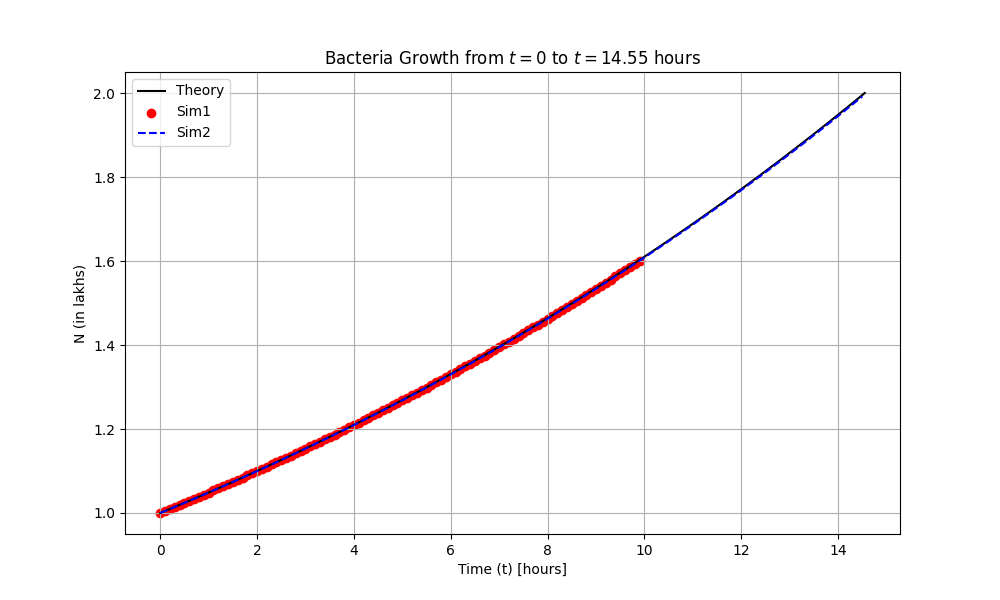
\includegraphics[width=\textwidth]{figs/plot.png} % Replace "filename" with your image file
    \caption{Plot}
\end{figure}



\end{document}
